%!TEX root = ../../report.tex

\chapter{Simulation} % (fold)
\label{cha:simulation}
This chapter is meant to answer the questions what, why and how a simulator takes part in the framework.
Starts with a motivation section \ref{sec:sim_motivation} which defines the scope of the simulator
 in the project, followed by a comparison of simulators \ref{sec:sim_comparison_of_simulators} and how to define a robot and its environment in it \ref{sec:robot_definition}; in the next section \ref{sec:robot_creation} is explained how the simulation model of the legs has been created and how to add new features, whilst the creation of the environment is dealt in the section \ref{sec:environment_creation}; finishes with a how-to dedicated section for launching the simulation from scratch in \ref{sec:how_to_simulate}.
%!TEX root = ../../../report.tex
\section{Motivation} % (fold)
\label{sec:sim_motivation}
What is a simulator, why to simulate

% section motivation (end)
%!TEX root = ../../../report.tex
\section{Comparison of simulators} % (fold)
\label{sec:sim_comparison_of_simulators}
When choosing a simulation platform there are several factors to have into account.
Three robotic simulators have been analyzed and compared. 
These are: LPZ Robots \cite{lpzrobots} (Figure \ref{fig:lpzrobots_example}), V-Rep \cite{vrep} (Figure \ref{fig:vrep_example}) and Gazebo \cite{gazebo} (Figure \ref{fig:gazebo_example}).
Some comparisons can be found in the literature as \cite{nogueiracomparative} or \cite{staranowicz2011survey} however the predominant criteria has been their integration with ROS.

\begin{figure}[hb!]
  \begin{subfigure}{.33\textwidth}
    \centering
    \includegraphics[width=.95\linewidth]{figures/vrep_example}
    \caption{V-Rep example}
    \label{fig:vrep_example}
  \end{subfigure}%
  \begin{subfigure}{.33\textwidth}
    \centering
    \includegraphics[width=.95\linewidth]{figures/lpzrobots_example}
    \caption{LPZ Robots example}
    \label{fig:lpzrobots_example}
  \end{subfigure}
  \begin{subfigure}{.33\textwidth}
    \centering
    \includegraphics[width=.95\linewidth]{figures/gazebo_example}
    \caption{Gazebo}
    \label{fig:gazebo_example}
  \end{subfigure}
  \caption{Simulation examples of the software analyzed}
  \label{fig:simulation_comparison}
\end{figure}

The RuBi robot is mainly targeted to be used in the AI department at the Maersk Mc-Kinney Møller Institute, where the toolbox GoRobots is being developed.
This is a set of tools, from a neuronal networks API to a genetic algorithm engine, written in C++ than is meant to be simulator-independent.
However, in order to provide a more general and supported simulation and development environment for the user, ROS Jade \cite{ros} has been selected as the tool to use.
The whole set of instruments provided in ROS along with its easy extendability give the opportunity to use the controllers and tools already developed in GoRobots.
Despite the fact that the three simulators compared have a C++ interface that would allow to interface them with ROS, Gazebo is already fully supported and integrated in ROS, making it the logic choice.
This reduces the learning curve of a new user and the installation process is easier due to it is included in the Open Source Robotics Foundation (OSRF) repositories.

Regarding the second condition, Gazebo has the feature of changing the physics engine in the beginning of the simulation, it has multiphysics support (fluids, electromagnetism...), it allows to load external geometries from STL or Collada and, the most important, has an active community behind it providing support and documentation. These are the reasons for selecting Gazebo as the simulator for the RuBi platform.
In \cite{physics_engine_gazebo_comparison}, a comparison with the different physical engines is carried out.
For the sake of simplicity the default one, Open Dynamics Engine (ODE), has been used, although the others have been tested.

% section comparison_of_simulators (end)\[
%!TEX root = ../../../report.tex
\section{Robot definition} % (fold)
\label{sec:robot_definition}
SDF vs URDF vs Xacro

% section robot_definition (end)
%!TEX root = ../../../report.tex
\section{Robot model creation} % (fold)
\label{sec:robot_creation}
One of the goals of the framework is to facilitate its further use and development.
For this reason this section is dedicated to explain how the robot model was created for Gazebo, so that it can be modified in the future.

A robot is defined as a set of links joined, where a link contains at least three blocks of information:
\begin{enumerate}
   \item The collision model: used to calculate the collisions with other agents in the simulation.
   \item The visual model: uniquely used for visual purposes.
   \item The inertial information: defines physical properties like the mass and the moments of inertia of the link.
\end{enumerate} 

A trade-off must be found for the precision of the collision model between accuracy and speed.
The more detailed is the model, the more accurate its simulation will become, but this implies a higher computational load and processing time.
The general advice is to have two simulation models: one for visual purposes and the other one for collisions.
In the case of the frame of RuBi the visual models are obtained directly by exporting the parts from SolidWorks, while the collision models are made out of primitive gazebo shapes (cubes, cylinders, spheres...) for the whole body except the feet.
Since the robot is not meant to collide with obstacles due to its nature and setup, the possible collisions in the body are not a priority, then each link is represented as a cylinder of the same length of the CAD model and of a radius enough to cover the whole part.
An example can be seen in the Figure \ref{fig:collision_model}.

The moments of inertia of each individual link are obtained directly from SolidWorks.
The CAD model includes the materials and thus the masses.
From these, the program is able to calculate the moments of inertia.
The Figure \ref{fig:moments_of_inertia} shows the representation of these parameters in the simulation.


\begin{figure}[hb!]
  \centering
  \begin{subfigure}{.45\textwidth}
    \centering
    \includegraphics[width=.5\linewidth]{figures/gazebo_collision_model.png}
    \caption{Gazebo showing the visual model, the moments of inertia and the collision model.}
    \label{fig:collision_model}
  \end{subfigure}
  \begin{subfigure}{.45\textwidth}
    \centering
    \includegraphics[width=.5\linewidth]{figures/gazebo_intertia_moments.png}
    \caption{Gazebo showing the visual model and the moments of inertia.}
    \label{fig:moments_of_inertia}
  \end{subfigure}
  \caption{Gazebo showing physical and visual propperties of RuBi.}
\end{figure}

It is essential to make sure that the visual models and moments of inertia are exported referred to the correct coordinate systems.
In the case of the ankle, for example, the STL file and the moments of inertia are calculated from the coordinate system whose origin is positioned in the middle of the rotational axis of the joint, with its Z axis attached to the rotational axis and Y pointing to the biggest extension of the part.
This can be seen in the Figure \ref{fig:solidworks_ankle_coodinate_system}.

\begin{figure}[ht!]
  \centering
  \includegraphics[width=0.75\linewidth]{figures/solidworks_ankle_coordinate_system}
  \caption{Coordinate system of the left ankle in SolidWorks.}
  \label{fig:solidworks_ankle_coodinate_system}
\end{figure}

Finally, in the Xacro file the information that lacks the URDF must be added in order to simulate with Gazebo.
To do so, the following has to be added to the RuBi description:
\begin{enumerate}
  \item \textbf{Plug-in for ROS Control}: Offers an interface for using ROS Control inside Gazebo.
  \item \textbf{Contact sensors}: Simulates contact sensors as in the feet of the real robot.
  \item \textbf{Friction coefficients}: Defines the friction between the feet and the floor.
\end{enumerate}

The robot has been simulated with direct drive transmission, since the springs configurations has not been implemented because of the lack of time.
This is left as further work.

% section robot_creation (end)
%!TEX root = ../../../report.tex
\section{Dimensional analysis} % (fold)
\label{sec:dimensional_analysis}
A problem came up when creating the robot. 
Some of the inertia moments obtained from SolidWorks, were in the order of magnitude of $10^{-8}$.
Such small number is not handled by the physics engine correctly causing the robot model to be unstable under normal conditions.

Three approaches were taken:
\begin{enumerate}
  \item \textbf{Change the physics engine}: As commented in the simulation comparison \ref{fig:simulation_comparison}, Gazebo supports multiple physics engines. Dart \cite{dart}, Simbody \cite{simbody}, Bullet \cite{bullet} and ODE \cite{ode}, where tested giving the same unstable behavior. 
  Thus, this method was discarded.
  \item \textbf{Fake the moments of inertia}: This would be to make 0 the really small moments of inertia and only leave the ones over a threshold.
  As the simulation is a qualitative analysis and no quantitative, an exact match of the moments of inertia is not needed. 
  \item \textbf{Dimensional analysis}: Based on \cite{dimensional_analysis}, the size of the robot can be increased in a proportion that make the figures big enough to be handled.
\end{enumerate}

Dimensional analysis can be applied to correlate the physical properties of the original robot with its scaled replica.
This is, if the original robot with mass $m$, volume $V$ and moment of inertia about an axis $I$, given a scale factor $s$, calculate the scaled replica $m'$, $V'$, $I'$ depending exclusively on $s$.

In the equation \ref{eq:general_inertia}, the generalized expression of the moment of inertia about an axis is shown.
\begin{equation}
\label{eq:general_inertia}
  I = \iiint_V \rho(u,v,w) |r^{2}| \,dx\,dy\,dz
\end{equation}

If the equation \ref{eq:general_inertia} is taken as the moment of inertia from the first link, the scaled one would be the shown in the equation \ref{eq:general_inertia_2}:
\begin{equation}
\label{eq:general_inertia_2}
  I' = \iiint_{V'} \rho(u,v,w)' |r^{'2}| \,dx'\,dy'\,dz'
\end{equation}

Supposing a scale factor of $s$ and as stated in the equations from \ref{eq:dx} to \ref{eq:dz}:

\begin{multicols}{3}
  \begin{equation}
  \label{eq:dx}
    \,dx=s \,dx'
  \end{equation}\break
  \begin{equation}
  \label{eq:dy}
    \,dy=s \,dy'
  \end{equation}\break
  \begin{equation}
  \label{eq:dz}
    \,dz=s \,dz'
  \end{equation}\break
\end{multicols}

Then can be deduced that $r$ increases proportionally with $s$ as shown in the figure \ref{fig:dimensional_analysis} and presented in the equation \ref{eq:dr}:
\begin{equation}
  \label{eq:dr}
  \,r=s \,r'
\end{equation}

\begin{figure}[ht!]
  \centering
  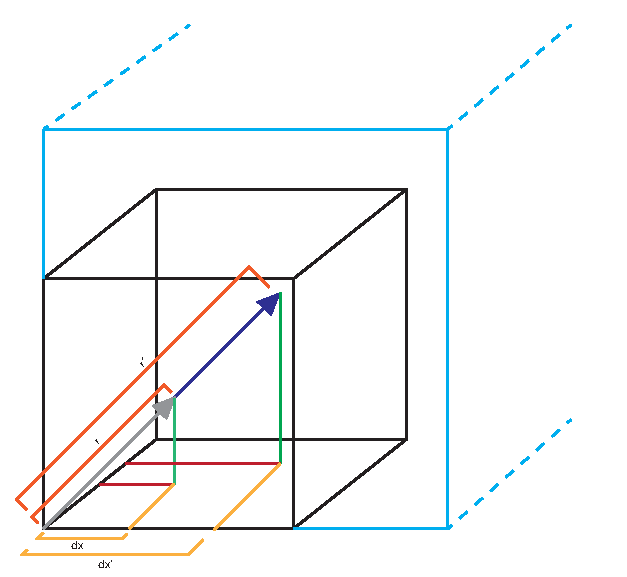
\includegraphics[width=0.5\linewidth]{figures/dimensional_analysis.pdf}
  \caption{Representation of a minimal volumentric cube.}
  \label{fig:dimensional_analysis}
\end{figure}

Assuming a constant density across all the scaled bodies, and particularizing for the moment of inertia of the center of gravity the moment of inertia is given then by \ref{eq:general_inertia_3}:
\begin{equation}
  \label{eq:general_inertia_3}
  I'_{CG} = \iiint_{V'} \rho(u,v,w)' |r^{'2}| \,dx'\,dy'\,dz' = s^{3} r_{CG}^{'2} m
\end{equation}

A correlation can be obtained for the inertia then as shown in \ref{eq:inertia_scale}:

\begin{equation}
\label{eq:inertia_scale}
  I' = \frac{s^{3} r_{CG}^{'2} m}{r_{CG}^{2} m} I = s^{5} I
\end{equation}

And lately the mass can be correlated as in \ref{eq:mass_scale}:
\begin{equation}
\label{eq:mass_scale}
  m' = V' \frac{m}{V} = s^{3}m
\end{equation}

As explained in the \ref{sec:robot_definition}, by using the Xacro format, mathematical expressions can be used.
The definition of the robot includes a set of variables in which is included $scale$ that is used to calculate $mass\_scaled$ and $inertia\_scaled$ that will modify the values of all the links to make a coherence scalable robot definition.

% section dimensional_analysis (end)
%!TEX root = ../../../report.tex
\section{Environment creation} % (fold)
\label{sec:environment_creation}
Talk about the rotational robot holder, the trade mill, other possible environment.

% section environment_creation (end)
%!TEX root = ../../../report.tex
\section{How to simulate} % (fold)
\label{sec:how_to_simulate}
The actions for starting the simulation are minimal and, with everything installed, just a terminal shall be opened and the user have to insert:

\begin{lstlisting}
roslaunch rubi_gazebo rubi_world.launch
\end{lstlisting}

The launch file will load ROS Control along with the simulation.
From that moment the user can run the controllers and the legs will move equally than in the real robot.
% section how_to_simulate (end)

% chapter simulation (end)
